\section{A Particle in an Infinite Square Well}
%By Matt Trawick

\makelabheader %(Space for student name, etc., defined in master.tex)

\bigskip

\begin{wrapfigure}[19]{r}{0.45\textwidth}
\begin{center}
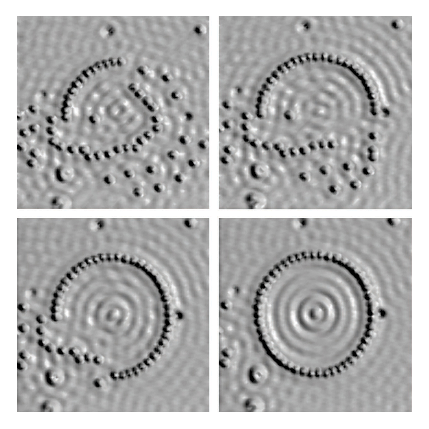
\includegraphics[width=0.42\textwidth]{particle_in_infinite_well/quantum_corral.eps}
\end{center}
\end{wrapfigure}

\textbf{Introduction}

The image on the right shows the step by step assembly of a ring of iron atoms on a smooth copper surface.  The  electrons on the surface of the copper are confined by the iron ring in a kind of ``quantum corral'' that highlights their wavelike nature. The apparent waves you see are areas of alternating high and low density of electrons, or more accurately \textit{probability density}.  Periodic areas of high and low probability density are a common feature anytime a particle is confined to a small space, as in an electron orbiting a single atomic nucleus.  Real atoms and electrons get pretty complicated pretty fast, so today you will use both a computer simulation and direct calculation to find regions of high and low probability for a much simpler, one-dimensional version of the situation shown in this picture.

Suppose that a particle (like an electron) is confined to move in only a single dimension, along the $x$ axis.  
The probability of finding the particle between any two points $x=a$ and $x=b$ is given by 
$P_{ab} = \int_a^b P(x)  \, dx$, where $P(x)$ is the \textit{probability density} of the particle at any specific location $x$.  The probability density is related to the \textit{wave function} $\psi(x)$ for the particle by 
$P(x)=\left|\psi(x)\right|^2$, thus the probability of finding the particle between $x=a$ and $x=b$ can be expressed as
$$P_{ab} = \int_a^b \left|\psi(x)\right|^2  \, dx.$$

\textbf{Activity 1: Wave Functions and Energy Quantization}
\begin{enumerate}[wide]
\item Consider a particle that is somehow constrained to move only in the $x$ direction.  It is also confined between the values of $x=0$ and $x=L$, and absolutely cannot move outside of that range.
(A macroscopic analogy for this particle in a ``one-dimensional box'' would be something like a fly stuck in a narrow glass tube that has been capped at both ends.)
\begin{enumerate}
\item What is $\psi(x)$ for $-\infty < x < 0$?
\answerspace{0.3in}

\item What is $\psi(x)$ for $L < x < \infty$?
\answerspace{0.3in}

\item What should $\displaystyle \int_{-\infty}^\infty \left|\psi(x)\right|^2  \, dx$ be?
\answerspace{0.3in}

\item Whatever the functional form of $\psi(x)$ is inside the box, what should its value be at $x=0$ and $x=L$ in order for 
$\psi(x)$ to be continuous?
\answerspace{0.3in}
\end{enumerate}
\end{enumerate}
\pagebreak

\begin{wrapfigure}[13]{r}{0.40\textwidth}
\begin{center}
\vspace{-0.2in}
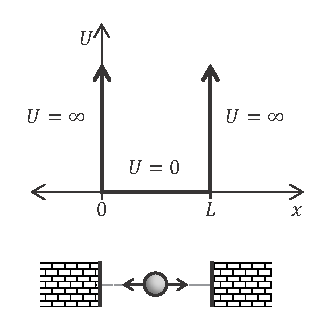
\includegraphics[width=0.34\textwidth]{particle_in_infinite_well/infinite_potential.eps}
\end{center}
\end{wrapfigure}

%A key aspect of the Schr\"odinger equation is the interplay between the energy of the particle $E$ and the potential energy function $U(x)$, which describes the forces acting on the particle.

To calculate $\psi(x)$, we'll first have to describe the forces acting on the particle using a potential energy function $U(x)$.
For our particle trapped in a box, the potential energy, shown on the right, is an energy ``well'': high on the outsides and low in the middle.  Because the side walls of the well are vertical, we call the potential a ``square well''.  If our particle absolutely cannot move beyond the vertical walls, our particle is in an ``infinite square well'', where outside the box $U(x)=\infty$, and inside the box $U(x)=0$.

\bigskip 
Within the range $0<x<L$, you can find $\psi(x)$ using the one-dimensional, time independent Schr\"odinger equation:
$$-\frac{\hbar^2}{2m} \frac{d^2\psi(x)}{dx^2} + U(x)\psi(x) = E\psi(x),$$
where $m$ is the mass of the particle, and the constant $\hbar$ (pronounced ``h-bar'') is related to our old friend Planck's constant $h$ by $\hbar = {h}/{2\pi} = 1.054 \times 10^{-34}~{\rm J} \cdot {\rm s}$.
\medskip
\begin{enumerate}[wide,resume]

\item What are some functions that satisfy the Schrödinger equation inside the 1-D box? (Here, the
Schr\"odinger equation says basically that the second derivative of a function is a bunch of constants times the negative of that same function.)
\answerspace{0.8in}

To give yourself a preview of what $\psi(x)$ looks like for different values of energy $E$, open the
following page in Firefox:
$$\verb!http://webphysics.davidson.edu/physletprob/ch10_modern/default.html!$$
Click on \button{Infinite Well} on the left hand side and let the Java applet run. This simulation shows a 1-dimensional box running from $x =-1.00$ to $x=+1.00$ (instead of from $x=0$ to $x=L$). The potential energy is shown as a red line at $U=0$, with the ``infinite'' vertical walls just off screen. Initially, your particle has been given an energy of $E=2.467$ (in some units), which leads to a function inside the box $\psi_{\rm in}(x)$ shown in blue. 

\item Draw sketches of the inside $\psi_{\rm in}(x)$ below for $E=2.467$, $E=6$, $E=10$, and $E=14$ or close to them.  You can type in a value of $E$ and press \button{Enter}.  (Notice that the $y$ axis of the graph of  $\psi_{\rm in}(x)$ shifts up as you increase the energy, as you can verify by trying $E=300$.  You can basically ignore this upward shift).
\answerspace{1.6in}

\item For the graphs that you just drew, 
%for the inside portion ψ_in (x), 
which values of $E$ come closest to producing a graph of $\psi(x)$ that is continuous everywhere, including at $x =+1.00$? Again, ignore the fact that different values of $E$ shift the graph's axes up and down, and understand that the zero of the vertical axis is always in the middle of the wave.  Also, remember that in this simulation the box length is from 
$x =-1.00$ to $x=+1.00$ instead of from 0 to $L$.)
\answerspace{0.3in}
\pagebreak[3]

\item Continue typing values for $E$ into the box, and find two more values of energy that produce continuous functions for $\psi(x)$.  At some point, when you tire of this game, you can play with typing in $n=2$ or $n=3$, and clicking on \button{find}. What are the lowest four values of $E$ that produce continuous functions for $\psi(x)$?
\answerspace{0.3in}

\item Draw quick sketches of $\psi(x)$ and $|\psi(x)|^2$ over the range $-\infty<x<\infty$ for $n=1$, $n=2$, and $n=3$.
\answerspace{2.8in}

\item The computer simulation showed you that to produce a continuous function for $\psi(x)$, only some values of $E$ are allowed. Now go back to the equations that you found in question 2, for a box extending from $x=0$ to $x=L$.  
\begin{enumerate}
\item If you wrote more than one function in question 2, only one of them will work now considering what has to happen at $x=0$.  Which one?
\answerspace{0.3in}

b) Your function should allow $x$ to be multiplied by a constant $k$.  What values must $k$ have such that $\psi_{\rm in}(x)$ is zero at $x=0$ and $x=L$?  
\answerspace{0.3in}
\end{enumerate}

\item Now use the Schr\"odinger equation and take the derivatives to write an expression for the allowed values of $E$ in terms of $h$, $m$, $L$, and some integer $n$.  
\answerspace{1.5in}

\textit{We have derived that the energy is quantized!  In classical mechanics we could give a particle any energy but in this case we see that if we are using quantum physics only discrete values of energy are possible!}

\pagebreak[3]

\textbf{Activity 2: Determining the Normalization Constant}

\item If you write the full wave function $\psi(x)$ for a particle in a 1-dimensional box, there is actually an arbitrary constant $A$ in front of it:
$$\psi(x)=A\sin kx$$
Use your answers to question 1 to find the value of $A$ (in terms of $L$) for $n=1$.  
Hint: you may find the following integral handy: $\int \sin^2ax \, dx = \frac{x}{2} -\frac{1}{4a}\sin 2ax $.
\answerspace{1.7in}

\item What's $A$ for $n=2$?  For $n=3$?  Do you see a pattern?
\answerspace{1.7in}

\item If your particle has $n=2$, what is the probability of finding it between $x=0$ and $x=0.25L$?  Is your calculated answer consistent with your pictures in question 6?
\answerspace{1.5in}

\item If your particle has $n=1$, what is the probability of finding it between $x=0$ and $x=0.25L$?  Again, is your calculated answer consistent with your pictures in question 6?
\answerspace{1.5in}

\end{enumerate}



